\documentclass[dcc]{fcfmcourse}
\usepackage{teoria}
\usepackage[utf8x]{inputenc}

\title{Tarea 1: Pilas de Arena}
\course[CC3001]{Algoritmos y Estructuras de Datos}
\professor{Nelson Baloian}
\professor{Patricio Poblete}
\assistant{Gabriel Azócar}
\assistant{Manuel Cáceres}
\assistant{Michel Llorens}
\assistant{Sergio Peñafiel}
% Si pasas el comando usedate a la clase, la fecha aparecerá bajo la lista de auxiliares.
% Puedes usar el formato de fecha por defecto de latex (y traducirla usando babel)
% o puedes escribir lo que quieras con el comando \date.
% \date{1 de Septiembre, 2015}

\setlength{\parindent}{0pt}

\begin{document}
\maketitle
\vspace{-2ex}
\begin{center}
Fecha de Entrega: 7 de Abril 23:59hrs
\end{center}

\begin{figure}[h!]
    \centering
    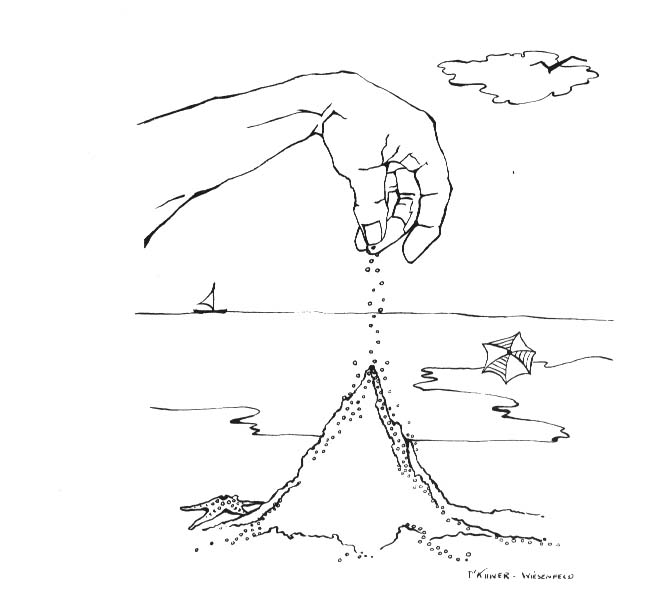
\includegraphics[scale=0.8]{imagenes/sanpile.jpg}
\end{figure}

\section{Introducción}
Muchas veces la descripción de problemas físicos puede ser complicada y los modelos analíticos que estos desprenden pueden llegar a ser imposibles de resolver usando las herramientas de cálculo convencionales. \\

Para este tipo de problema es común recurrir a la ayuda de una modelación computacional junto con un algoritmo que describa o aproxime las leyes físicas. Los resultados, si bien son aproximaciones, pueden dar un buen indicio del comportamiento real del problema. \\

En esta tarea se estudiará el fenómeno de granos de arena apilados en el espacio, a estos se les aplicará una regla de estabilidad por gravedad y se visualizarán las estructuras resultantes.

\section{Explicación}

\subsection{Pilas de Arena}
Para comenzar el modelamiento se tiene una superficie plana potencialmente infinita donde se depositarán los granos de arena. La superficie se discretizará en celdas cuadradas de igual tamaño y forma generando una malla como se muestra en la figura siguiente.

\begin{figure}[!ht]
    \centering
    
\includegraphics[scale=0.5]{imagenes/grid.png}
\end{figure}

En cada celda se tendrá información de cuantos granos de arena apilados hay en esa celda. Así por ejemplo la siguiente configuración indica que en la celda central hay una pila de 5 granos en la superior hay 2, y a la derecha 1. El resto no contiene granos de arena.

\begin{figure}[!ht]
    \centering
    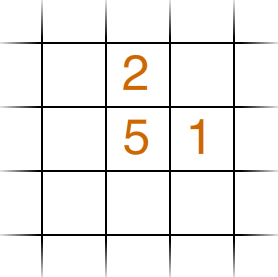
\includegraphics[scale=0.5]{imagenes/gridex1.png}
\end{figure}

Dado que las celdas de la grilla representan regiones del espacio muy pequeñas, es posible pensar que no podemos tener una cantidad muy grande de granos apilados en una misma celda dado que este sistema se volvería inestable. Para este modelo supondremos que cuando existen 4 o más granos de arena en una celda, entonces esta se desborda dejando un grano en cada una de las celdas vecinas (arriba, abajo, derecha e izquierda). De esta forma el ejemplo anterior sería inestable y al aplicar la regla quedaría en la configuración que se muestra en la figura.

\begin{figure}[!ht]
    \centering
    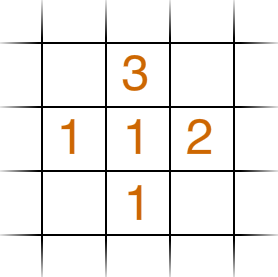
\includegraphics[scale=0.5]{imagenes/gridex2.png}
\end{figure}

\newpage
Bajo este principio, un problema surge al tener más de una celda inestable pues no se especifica a cuál debe aplicarse la regla primero, sin embargo es posible demostrar que el dominio definido junto con la regla anterior generan un grupo \textbf{abeliano} lo cual nos indica que si existen 2 celdas A y B inestables, aplicar la regla sobre A y luego sobre B genera el mismo resultado que haberla aplicado sobre B y luego A. Luego el orden en que se apliquen las reglas no es relevante.


\subsection{Visualización}

Para esta tarea dispondrá de la clase \texttt{Ventana} que le ayudará en la visualización. La definición es la siguiente. \\

\def\arraystretch{1.8}
\begin{tabular}{|p{0.45\textwidth}|p{0.48\textwidth}|} \hline

\texttt{Ventana(int tamaño, String titulo)} & Constructor, crea y muestra una nueva ventana vacía cuadrada del tamaño y titulo especificados como parámetros. \\ \hline

\texttt{mostrarMatriz(int[][] mat)} & Dibuja en la ventana la matriz indicada como cuadros de colores. Esta debe contener valores entre 0 y 3 (ambos incluidos).
 \\ \hline
\end{tabular}

\newpage
\section{Implementación}
En esta tarea usted deberá entregar un archivo \texttt{PilaArena.java} que hará una simulación de las pilas de arenas descritas anteriormente, en particular simularemos las estructuras que se generan al estabilizar una pila de granos muy alta en una única celda. \\

Para esto cree un programa que realice lo siguiente:

\begin{enumerate}
    \item Pida al usuario un entero N que indica la cantidad de granos que se depositarán en el centro.
    \item Cree una matriz de enteros de un tamaño apropiado. Esta describirá los granos de arena en cada celda. Por esto debe inicializarla con 0 excepto en la celda central cuyo valor debe ser N.
    \item Aplique la regla de estabilidad, para esto primero debe ver celda a celda si es necesario aplicar la regla de desborde o no, repita este procedimiento hasta que el sistema completo sea estable.
    \item Cree una ventana usando la clase provista y muestre la matriz resultante en pantalla.
\end{enumerate}

En la imagen siguiente se muestra el resultado esperado usando N = 100000. El cual tomó cerca de 30s en ejecutarse.

\begin{figure}[!ht]
    \centering
    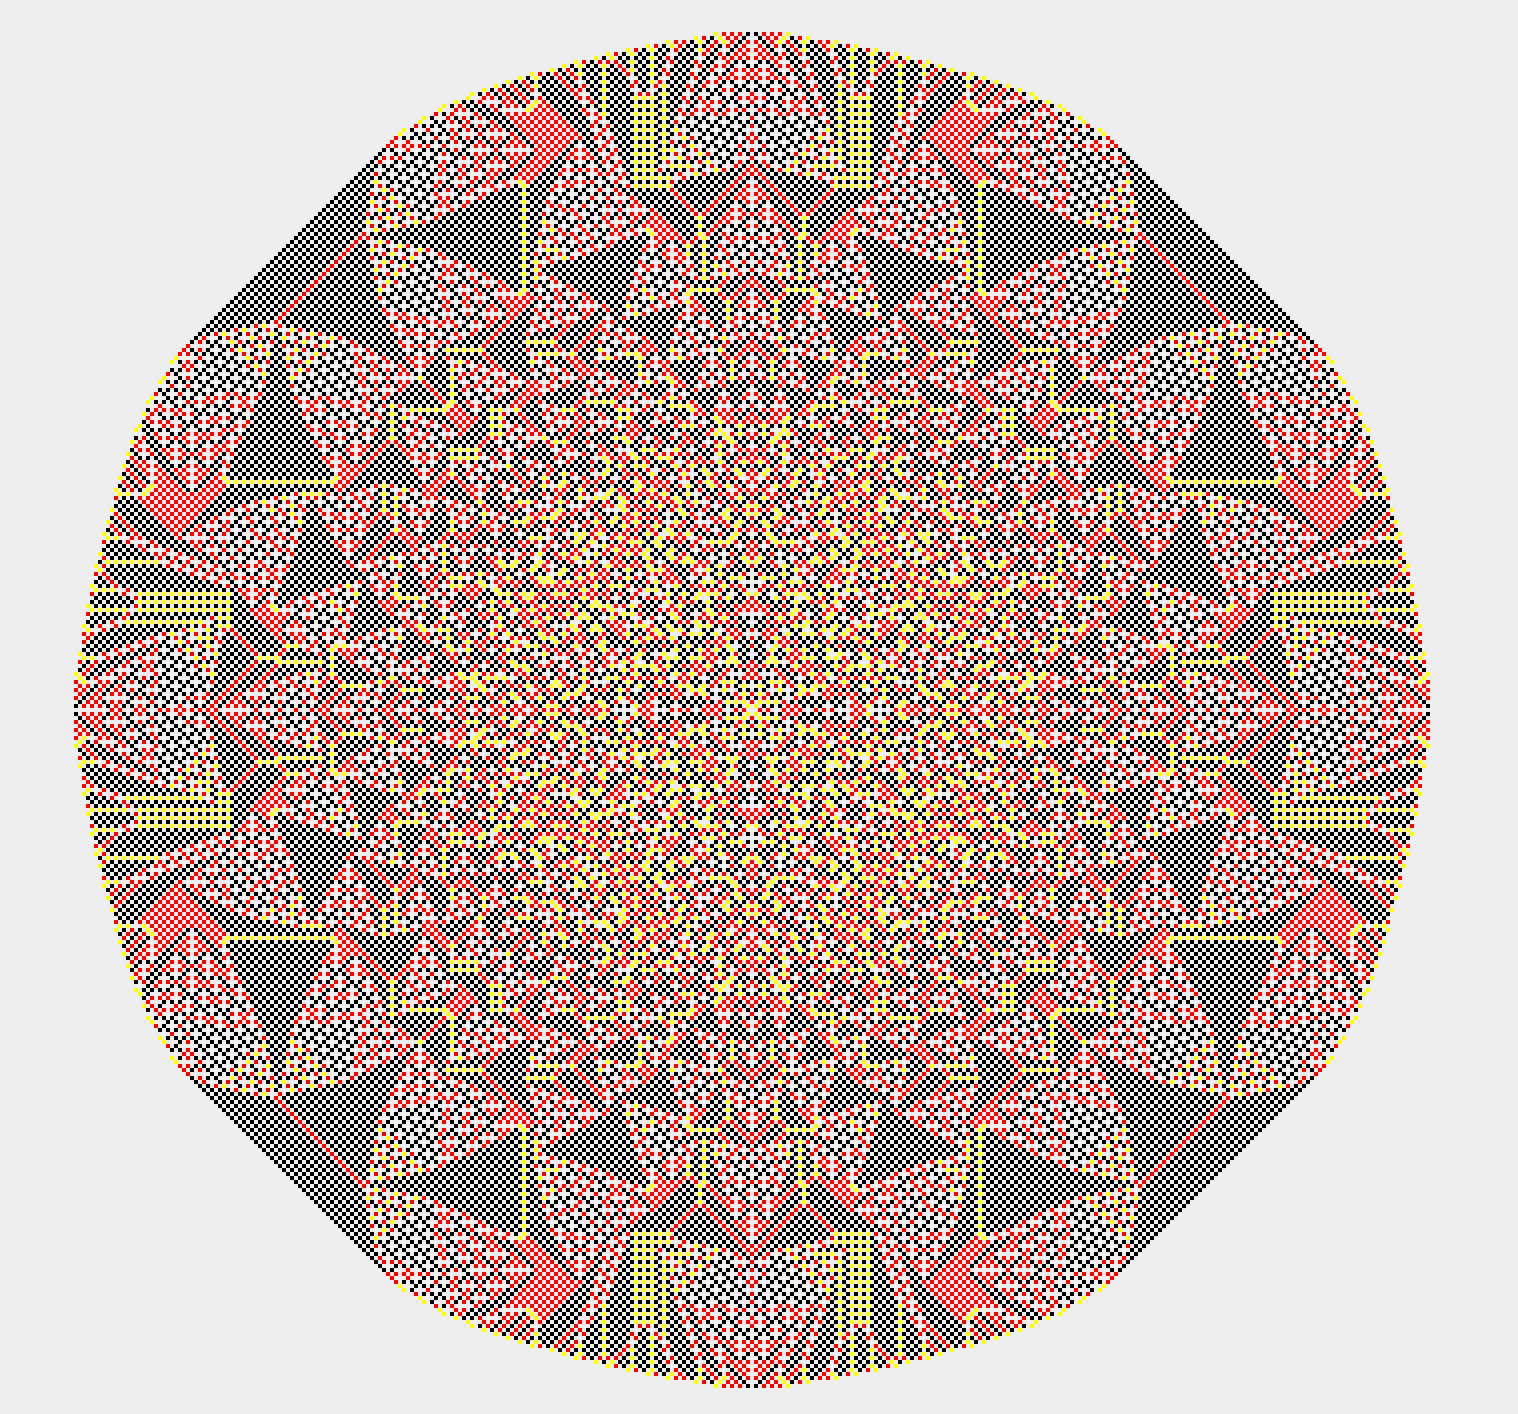
\includegraphics[scale=0.7]{imagenes/res.png}
\end{figure}

\subsection*{Caso de borde}

Dado que en el modelo original la matriz es potencialmente infinita no hay problema con el desborde pues siempre existen vecinos a una celda. En la implementación anterior, la matriz es finita y los bordes no tienen todos sus vecinos, por lo tanto debe considerar este caso en su solución y explicarlo en el informe. \\

Algunas soluciones válidas son: 

\begin{itemize}
    \item Dado el valor de N encontrar una cota superior para el tamaño de la matriz, justificándolo en el informe.
    \item Suponer que el borde es un sumidero y por lo tanto siempre tiene valor 0 aun cuando le lleguen granos.
    \item Si se necesita más espacio en la matriz, copiarla a una de tamaño más grande y seguir iterando.
\end{itemize}

No es aceptable que el programa no responda si ocurre este caso.  

\newpage
\section{Reglas}

\begin{itemize}
    \item Esta tarea debe ser resuelta en Java.
    \item Es obligatorio la entrega de un informe en formato pdf junto con su tarea (Ver siguiente sección).
    \item Esta tarea es de carácter individual, cualquier caso de copia se evaluará con la nota mínima.
    \item No olvide subir a U-cursos \textbf{todos} los archivos necesarios para que su tarea funcione correctamente.
    \item Debe subir los archivos de código fuente (*.java). Los archivos compilados (*.class) no serán evaluados.
    \item Cualquier duda respecto a la tarea puede ser consultada usando el foro del curso.
    \item No se aceptan atrasos.
\end{itemize}

\section{Informe}

El informe debe describir el trabajo realizado, el código fuente desarrollado, los resultados obtenidos y las conclusiones o interpretaciones de estos. Principalmente sea conciso, describiendo cada uno de los puntos que a continuación se indican.

\begin{itemize}
    \item \textbf{Portada:} Indicando número de la tarea, fecha, autor, email, código del curso.
    \item \textbf{Introducción:} Descripción breve del problema y su solución.
    \item \textbf{Análisis del problema:} Exponga en detalle el problema, los supuestos que pretende ocupar, casos de borde y brevemente la metodología usada para resolverlo.
    \item \textbf{Solución del problema:}
    \begin{itemize}
        \item Algoritmos de solución, incluyendo toda la información y figuras que considere necesarias.
        \item Partes relevantes del código fuente
        \item Ejemplos de entradas y salidas escogidos por usted.
    \end{itemize}
    \item \textbf{Modo de uso:} explicando brevemente cualquier dato extra necesario para la compilación y ejecución de su programa.
    \item \textbf{Resultados y análisis:} Todo el análisis de los resultados, los gráficos, imágenes y la discusión requerida.
\end{itemize}

\end{document}
